
\documentclass[a4paper,11pt]{article}
\usepackage[a4paper, margin=8em]{geometry}

% usa i pacchetti per la scrittura in italiano
\usepackage[french,italian]{babel}
\usepackage[T1]{fontenc}
\usepackage[utf8]{inputenc}
\frenchspacing 

% usa i pacchetti per la formattazione matematica
\usepackage{amsmath, amssymb, amsthm, amsfonts}

% usa altri pacchetti
\usepackage{gensymb}
\usepackage{hyperref}
\usepackage{standalone}

\usepackage{colortbl}

\usepackage{xstring}
\usepackage{karnaugh-map}

% imposta il titolo
\title{Appunti Calcolatori Elettronici}
\author{Luca Seggiani}
\date{2025}

% imposta lo stile
% usa helvetica
\usepackage[scaled]{helvet}
% usa palatino
\usepackage{palatino}
% usa un font monospazio guardabile
\usepackage{lmodern}

\renewcommand{\rmdefault}{ppl}
\renewcommand{\sfdefault}{phv}
\renewcommand{\ttdefault}{lmtt}

% circuiti
\usepackage{circuitikz}
\usetikzlibrary{babel}

% testo cerchiato
\newcommand*\circled[1]{\tikz[baseline=(char.base)]{
\node[shape=circle,draw,inner sep=2pt] (char) {#1};}}

% disponi il titolo
\makeatletter
\renewcommand{\maketitle} {
	\begin{center} 
		\begin{minipage}[t]{.8\textwidth}
			\textsf{\huge\bfseries \@title} 
		\end{minipage}%
		\begin{minipage}[t]{.2\textwidth}
			\raggedleft \vspace{-1.65em}
			\textsf{\small \@author} \vfill
			\textsf{\small \@date}
		\end{minipage}
		\par
	\end{center}

	\thispagestyle{empty}
	\pagestyle{fancy}
}
\makeatother

% disponi teoremi
\usepackage{tcolorbox}
\newtcolorbox[auto counter, number within=section]{theorem}[2][]{%
	colback=blue!10, 
	colframe=blue!40!black, 
	sharp corners=northwest,
	fonttitle=\sffamily\bfseries, 
	title=Teorema~\thetcbcounter: #2, 
	#1
}

% disponi definizioni
\newtcolorbox[auto counter, number within=section]{definition}[2][]{%
	colback=red!10,
	colframe=red!40!black,
	sharp corners=northwest,
	fonttitle=\sffamily\bfseries,
	title=Definizione~\thetcbcounter: #2,
	#1
}

% disponi codice
\usepackage{listings}
\usepackage[table]{xcolor}

\definecolor{codegreen}{rgb}{0,0.6,0}
\definecolor{codegray}{rgb}{0.5,0.5,0.5}
\definecolor{codepurple}{rgb}{0.58,0,0.82}
\definecolor{backcolour}{rgb}{0.95,0.95,0.92}

\lstdefinestyle{codestyle}{
	backgroundcolor=\color{black!5}, 
	commentstyle=\color{codegreen},
	keywordstyle=\bfseries\color{magenta},
	numberstyle=\sffamily\tiny\color{black!60},
	stringstyle=\color{green!50!black},
	basicstyle=\ttfamily\footnotesize,
	breakatwhitespace=false,         
	breaklines=true,                 
	captionpos=b,                    
	keepspaces=true,                 
	numbers=left,                    
	numbersep=5pt,                  
	showspaces=false,                
	showstringspaces=false,
	showtabs=false,                  
	tabsize=2
}

\lstdefinestyle{shellstyle}{
	backgroundcolor=\color{black!5}, 
	basicstyle=\ttfamily\footnotesize\color{black}, 
	commentstyle=\color{black}, 
	keywordstyle=\color{black},
	numberstyle=\color{black!5},
	stringstyle=\color{black}, 
	showspaces=false,
	showstringspaces=false, 
	showtabs=false, 
	tabsize=2, 
	numbers=none, 
	breaklines=true
}


\lstdefinelanguage{assembler}{ 
	keywords={AAA, AAD, AAM, AAS, ADC, ADCB, ADCW, ADCL, ADD, ADDB, ADDW, ADDL, AND, ANDB, ANDW, ANDL,
		ARPL, BOUND, BSF, BSFL, BSFW, BSR, BSRL, BSRW, BSWAP, BT, BTC, BTCB, BTCW, BTCL, BTR, 
		BTRB, BTRW, BTRL, BTS, BTSB, BTSW, BTSL, CALL, CBW, CDQ, CLC, CLD, CLI, CLTS, CMC, CMP,
		CMPB, CMPW, CMPL, CMPS, CMPSB, CMPSD, CMPSW, CMPXCHG, CMPXCHGB, CMPXCHGW, CMPXCHGL,
		CMPXCHG8B, CPUID, CWDE, DAA, DAS, DEC, DECB, DECW, DECL, DIV, DIVB, DIVW, DIVL, ENTER,
		HLT, IDIV, IDIVB, IDIVW, IDIVL, IMUL, IMULB, IMULW, IMULL, IN, INB, INW, INL, INC, INCB,
		INCW, INCL, INS, INSB, INSD, INSW, INT, INT3, INTO, INVD, INVLPG, IRET, IRETD, JA, JAE,
		JB, JBE, JC, JCXZ, JE, JECXZ, JG, JGE, JL, JLE, JMP, JNA, JNAE, JNB, JNBE, JNC, JNE, JNG,
		JNGE, JNL, JNLE, JNO, JNP, JNS, JNZ, JO, JP, JPE, JPO, JS, JZ, LAHF, LAR, LCALL, LDS,
		LEA, LEAVE, LES, LFS, LGDT, LGS, LIDT, LMSW, LOCK, LODSB, LODSD, LODSW, LOOP, LOOPE,
		LOOPNE, LSL, LSS, LTR, MOV, MOVB, MOVW, MOVL, MOVSB, MOVSD, MOVSW, MOVSX, MOVSXB,
		MOVSXW, MOVSXL, MOVZX, MOVZXB, MOVZXW, MOVZXL, MUL, MULB, MULW, MULL, NEG, NEGB, NEGW,
		NEGL, NOP, NOT, NOTB, NOTW, NOTL, OR, ORB, ORW, ORL, OUT, OUTB, OUTW, OUTL, OUTSB, OUTSD,
		OUTSW, POP, POPL, POPW, POPB, POPA, POPAD, POPF, POPFD, PUSH, PUSHL, PUSHW, PUSHB, PUSHA, 
		PUSHAD, PUSHF, PUSHFD, RCL, RCLB, RCLW, MOVSL, MOVSB, MOVSW, STOSL, STOSB, STOSW, LODSB, LODSW,
		LODSL, INSB, INSW, INSL, OUTSB, OUTSL, OUTSW
		RCLL, RCR, RCRB, RCRW, RCRL, RDMSR, RDPMC, RDTSC, REP, REPE, REPNE, RET, ROL, ROLB, ROLW,
		ROLL, ROR, RORB, RORW, RORL, SAHF, SAL, SALB, SALW, SALL, SAR, SARB, SARW, SARL, SBB,
		SBBB, SBBW, SBBL, SCASB, SCASD, SCASW, SETA, SETAE, SETB, SETBE, SETC, SETE, SETG, SETGE,
		SETL, SETLE, SETNA, SETNAE, SETNB, SETNBE, SETNC, SETNE, SETNG, SETNGE, SETNL, SETNLE,
		SETNO, SETNP, SETNS, SETNZ, SETO, SETP, SETPE, SETPO, SETS, SETZ, SGDT, SHL, SHLB, SHLW,
		SHLL, SHLD, SHR, SHRB, SHRW, SHRL, SHRD, SIDT, SLDT, SMSW, STC, STD, STI, STOSB, STOSD,
		STOSW, STR, SUB, SUBB, SUBW, SUBL, TEST, TESTB, TESTW, TESTL, VERR, VERW, WAIT, WBINVD,
	XADD, XADDB, XADDW, XADDL, XCHG, XCHGB, XCHGW, XCHGL, XLAT, XLATB, XOR, XORB, XORW, XORL},
	keywordstyle=\color{blue}\bfseries,
	ndkeywordstyle=\color{darkgray}\bfseries,
	identifierstyle=\color{black},
	sensitive=false,
	comment=[l]{\#},
	morecomment=[s]{/*}{*/},
	commentstyle=\color{purple}\ttfamily,
	stringstyle=\color{red}\ttfamily,
	morestring=[b]',
	morestring=[b]"
}

\lstset{language=assembler, style=codestyle}

% disponi sezioni
\usepackage{titlesec}

\titleformat{\section}
{\sffamily\Large\bfseries} 
{\thesection}{1em}{} 
\titleformat{\subsection}
{\sffamily\large\bfseries}   
{\thesubsection}{1em}{} 
\titleformat{\subsubsection}
{\sffamily\normalsize\bfseries} 
{\thesubsubsection}{1em}{}

% tikz
\usepackage{tikz}

% float
\usepackage{float}

% grafici
\usepackage{pgfplots}
\pgfplotsset{width=10cm,compat=1.9}

% disponi alberi
\usepackage{forest}

\forestset{
	rectstyle/.style={
		for tree={rectangle,draw,font=\large\sffamily}
	},
	roundstyle/.style={
		for tree={circle,draw,font=\large}
	}
}

% disponi algoritmi
\usepackage{algorithm}
\usepackage{algorithmic}
\makeatletter
\renewcommand{\ALG@name}{Algoritmo}
\makeatother

% disponi numeri di pagina
\usepackage{fancyhdr}
\fancyhf{} 
\fancyfoot[L]{\sffamily{\thepage}}

\makeatletter
\fancyhead[L]{\raisebox{1ex}[0pt][0pt]{\sffamily{\@title \ \@date}}} 
\fancyhead[R]{\raisebox{1ex}[0pt][0pt]{\sffamily{\@author}}}
\makeatother

\begin{document}
% sezione (data)
\section{Lezione del 06-05-25}

% stili pagina
\thispagestyle{empty}
\pagestyle{fancy}

% testo
Riprendiamo più nel dettaglio i concetti che abbiamo solamente accennatto alla scorsa lezione.

\subsubsection{Ordinamento delle istruzioni}
Abbiamo che l'\textit{ordinamento totale} delle istruzioni del programma è solo un artefatto di come questo è compilato: non necessariamente le istruzioni vanno eseguite in tale ordine per arrivare allo stesso risultato finale.

Le istruzioni si trovano infatti solo in un \textit{ordinamento parziale}, dove solo alcune istruzioni hanno bisogno, per motivi di sincronia, di essere eseguite successivamente ad altre.

Prendiamo quindi l'esempio \lstinline|op1, src1, sec2, dst|, con sintassi simile all'assembly ARM (e in generale delle istruzioni RISC, dove ricordiamo gli operandi sono sempre registri). 
Una volta che i sorgenti \lstinline|src1| e \lstinline|src2| sono definiti, questa può essere eseguita.

Ipotizziamo quindi un'architettura dove sono previste un numero arbitrario di ALU, preceduta da componenti che denominiamo \textbf{stazioni di prenotazione}, fondamentalmente registri capaci di contenere la codifica macchina di una istruzione.

Ogni istruzione che viene decodificata dal processore viene spostata in una stazione di prenotazione. 
Non appena gli operandi saranno pronti, l'istruzione potrà quindi essere messa in esecuzione.

Viene da sé che questa architettura ci permette di ottenere un'esecuzione delle istruzioni che è \textit{fuori ordine} e in \textit{parallelo}.

\par\smallskip

Vediamo quindi nel dettaglio lo schema funzionale del Pentium Pro:
\begin{center}
	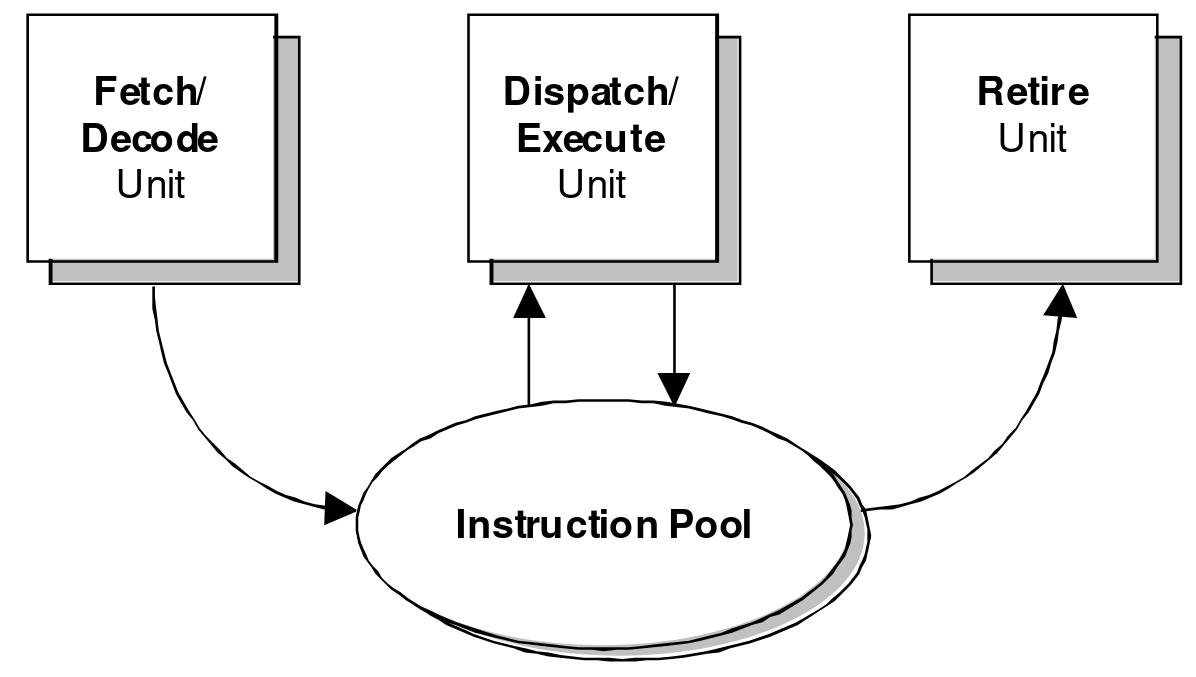
\includegraphics[scale=.33]{../figures/ppro_hilevel.png}
\end{center}

I 3 blocchi funzionali si occupano rispettivamente di:
\begin{enumerate}
	\item \textbf{Fetch/Decode} Unit: come abbiamo detto in 24.1.3, si occupa di convertire le istruzioni CISC in micro-operazioni RISC da 4 KiB ciascuna.
		Le istruzioni CISC più complesse fornite dall'instruction set x86 vengono tradotte in 2 o più micro-operazioni.
		
		Le micro-operazioni vengono poi introdotte nella cosiddetta \textbf{instruction pool}, cioè una struttura che mantiene le micro-operazioni decodificate.
		L'instruction pool viene riempita con un certo grado di \textit{look-ahead}, cioè si ottengono, in maniera speculativa, istruzioni successive al punto di esecuzione corrente.

		Infine, notiamo che nella pratica l'instruction pool viene implementata da un buffer detto \textbf{ROB}, \textit{Reorder Buffer};

	\item \textbf{Dispatch/Execute} Unit: si occupa di prelevare le istruzoni dal ROB ed effettuarne il \textit{dispatch} (\textbf{emissione}) all'interno delle stazioni di prenotazione.
		Queste si occupano quindi di eseguire l'istruzione ottenuta, secondo le regole sulle dipendenze che vedremo fra poco, e probabilmente attraverso l'arbitrio di una qualche unità di controllo superiore;

	\item \textbf{Retire} Unit: questo è il componente finale della catena, che si occupa di prelevare dal ROB le istruzioni terminate, ed effettuarne il \textbf{ritiro} nell'ordine in cui sono state scritte dal programmatore.
\end{enumerate}

\subsubsection{Dipendenze}
Chiaramente, resterà da definire le regole secondo le quali le istruzioni devono essere eseguite prima o dopo di altre nello schema di esecuzione fuori ordine.
Chiamiamo queste condizioni \textbf{dipendenze}, fra cui distinguiamo:
\begin{itemize}
	\item Dipendenze \textbf{dati};
	\item Dipendenze \textbf{nomi};
	\item Dipendenze \textbf{controllo};
\end{itemize}
dove la prima e l'ultima non vanno confuse con le alee: adesso parliamo di conseguenze di come è fatto il \textit{programma}, non di come è fatto il \textit{processore}.

Le dipendenze \textbf{dati} sono il caso che abbiamo già visto.
Se abbiamo due istruzioni:
\begin{lstlisting}	
add r1, r2, r3
...
sub r4, r3, r5
\end{lstlisting}
si ha che la \lstinline|sub| dipende per dati dalla \lstinline|add|, in quanto questa intacca \lstinline|r3|, operando.

Per ogni registro dovremo quindi mantenere delle informazioni associate: quando una istruzione viene messa in una stazione (si dice viene \textbf{emessa}), si alza un certo flag associato al registro che intaccherà. 
Questo flag viene poi abbassato in fase di esecuzione vera e propria, insieme all'aggiornamento dei dati del registro stesso.
Un istruzione successiva che vuole usare tale registro dovrà quindi controllare tale flag per capire se quell'operando è pronto.

Le dipendenze sui \textbf{nomi} si dividono in due categorie:
\begin{itemize}
	\item \textbf{Antidipendenze}:
	Poniamo di avere le due istruzioni:
\begin{lstlisting}
add r1, r2, r3
...
sub r4, r5, r1
\end{lstlisting}
in questo caso non si può eseguire la \lstinline|sub| prima della \lstinline|add|, in quanto la prima necessita del \textit{vecchio} contenuto di \lstinline|r1|, non quello che avremo dopo la \lstinline|sub|.
Si deve quindi evitare di mettere in attesa la \lstinline|sub| finché la \lstinline|add| non è conosciuta.

Per risolvere questo tipo di dipendenza dovremmo quindi dotare ogni registro, oltre al flag W, un contatore C che conti quante stazioni contengono istruzioni che usano quel registro come sorgente.
Ogni istruzione emessa alza i contatori dei suoi sorgenti, e ogni istruzione eseguita fino in fondo li abbassa.
Avremo quindi che un istruzione potrà scrivere sulla sua destinazione quando il numero di lettori, e quindi il contatore, è pari a 0.

	\item Dipendenze in \textbf{uscita}:
		Poniamo di avere le due istruzioni:
\begin{lstlisting}
add r1, r2, r3
...
sub r4, r5, r3
\end{lstlisting}
che può sembrare strano, ma può succedere nel caso qualcuno usi \lstinline|r3| fra le due istruzioni, o il compilatore lo faccia comunque per motivi di ottimizzazione.
Ad esempio questo succede spesso per quanto riguarda il registro dei flag, che viene aggiornato costantemente ma letto solamente dalle istruzioni di salto. 

Per risolvere questo tipo di dipendenze si controlla il flag associato al registro di uscita prima dell'emissione: in caso questo sia già preso in scrittura si mette l'istruzione in attesa (simile alle bolle che avevamo visto per la pipeline), per poi emetterla solo quando \lstinline|r3| è stato modificato. 
\end{itemize}

Possiamo dire che, date due istruzioni $a$, $b$ da eseguire in quest'ordine, le dipendenze si classificano come nel seguente schema:

\begin{table}[h!]
	\center
	\begin{tabular} { c | c  c  }
		& $a$ in scrittura & $a$ in lettura \\ 
		\hline
		$b$ in scrittura & Dipendenza in uscita & Antidipendenza \\ 
		$b$ in lettura & Dipendenza sui dati & // 
	\end{tabular}
\end{table}

Le dipendenze sul \textbf{controllo} si verificano quando istruzioni possono o meno essere eseguito sulla base dell'esito di istruzioni di salto.
Ad esempio, preso:
\begin{lstlisting}	
	cmp
	ja fine

	add ...
	sub ...

fine:
	mul ...
\end{lstlisting}
vorremo che le \lstinline|add| e \lstinline|sub| non fossero eseguite in caso positivo della \lstinline|ja|, mentre la \lstinline|mul| venga eseguita comunque.
Chiaramente questo non è facile, in quanto potremmo avere:
\begin{lstlisting}	
	cmp
	ja fine

	add ...
	sub ...

	jmp fine2

fine:
	mul ...

fine2:
\end{lstlisting}
dove la \lstinline|mul| non può essere eseguita comunque, ma questo non si può sapere finché non si entra nel blocco \lstinline|add ... sub|.
Il processore non ha quindi speranze per risolvere il problema, se non assumere \textit{per eccesso} che tutto ciò che viene dopo la jump dipende dalla jump. 

\subsubsection{Traduzione da CISC a RISC}
Vediamo come può essere effettuata la traduzione da un istruzione CISC al corrispondente insieme di istruzioni \lstinline|RISC|.
Prendiamo ad esempio:
\begin{lstlisting}[language=C++, style=codestyle]	
add %rax, 1000(%ebx, %ecx, 8)
\end{lstlisting}
questa dovrà essere tradotta in qualcosa come:
\begin{lstlisting}[language=C++, style=codestyle]	
shl %ecx, $3, tmp1
add %ebx, tmp1, tmp1
ld 1000(tmp1), tmp2
add %rax, tmp2, tmp2
st tmp2, 1000(tmp1)
\end{lstlisting}

Vediamo come abbiamo bisogno di registri dedicati, \lstinline|tmp1| e \lstinline|tmp2|, interni al processore e non accessibili al programmatore.
Questo chiaramente perchè non vogliamo che la trasformazione in RISC delle istruzioni CISC sporchi i registri programmatore.

\subsubsection{Registri fisici}
Dotando il processore di più registri fisici, oltre a quelli programmatore, possiamo rimuovere le dipendenze sui nomi, dette anche \textit{false dipendenze}. 

Questo si fa attraverso il meccanismo di \textbf{rinominazione} dei registri.
Facciamo in modo che ogni registro logico punti ad un registro fisico, con il numero di registri fisici anche maggiore di quello dei registri logici.

Quando il processore incontra un'istruzione, chiama un registro fisico non appena usato come come il registro di uscita (per tutti, non solo per se stesso), e prende i registri fisici puntati dai registri logici sorgenti come registri sorgenti.
Ad esempio, assunto di partire da una mappatura identità, prendiamo l'istruzione:
\begin{lstlisting}	
add r1, r2, r3
\end{lstlisting}
che viene trasformata in:
\begin{lstlisting}	
add f1, f2, f6 # assunto f6 libero
\end{lstlisting}
dove \textit{libero} significa non usati per niente, quindi non puntati e con contatore C e flag W a 0.

Notiamo che questa fase di traduzione si svolge \textit{dopo} la fase di traduzione in RISC effettuata nei componenti addetti alla fetch e decode, e quindi solo in fase di emissione.

Abbiamo quindi rimosso tutti gli stalli necessari alle dipendenze fra i nomi (le cosiddette \textit{false dipendenze}), in quanto ogni istruzione emessa ha come destinazione un registro fisico libero.

Un'istruzione che ha già avuto i suoi registri logici sorgenti tradotti in registri fisici non si preoccupa di ulteriori aggiornamenti ai registri sorgenti, in quanto queste verranno fatte su altri registri, liberi, e non su quelli che lei ha scelto.

\par \medskip

Vediamo quindi come usare il meccanismo di ridenominazione dei registri per risolvere anche gli stalli sulle dipendenze di controllo.

Avevamo già introdotto l'esecuzione speculativa delle istruzioni.
Nella terminologia Intel, questa viene eseguita attraverso un \textbf{ROB}, \textit{Reorder Buffer}.
All'interno del Reorder Buffer viene mantenuta una lista ordinata delle istruzioni, assieme ad un flag che indica che quell'istruzione è terminata (ma non che il risultato è stato scritto!).

Prima di un'istruzione di salto, si possono eseguire e ritirare tutte le istruzioni.
Dopo l'istruzione di salto, immaginiamo che le istruzioni successive vengano eseguite ma non ritirate (scritte nei registri fisici), secondo una predizione fatta come descritto in 24.1.2.
A seguito del salto, potremmo quindi verificare se la predizione è stata corretta: in caso di hit, avremo che potremo ritirare le istruzioni già eseguite, altrimenti dovremo svuotare il Reorder Buffer.

In ogni caso, informazioni più dettagliate sul funzionamento dell'esecuzione fuori ordine nel Pentium Pro si possono trovare nel manuale dello stesso, reperibile al link: \url{https://download.intel.com/design/PentiumII/manuals/24400101.pdf}.

\newpage

\end{document}
